\chapter{Background}
\label{ch:background}

% the code below specifies where the figures are stored
\ifpdf
    \graphicspath{{chapters/ch2_figures/PNG/}{chapters/ch2_figures/PDF/}{chapters/ch2_figures/}}
\else
    \graphicspath{{chapters/ch2_figures/EPS/}{chapters/ch2_figures/}}
\fi


% ----------------------------------------------------------------------
%: ----------------------- content ----------------------- 
% ----------------------------------------------------------------------

\section{Diagnosis and Treatment of Neocortical Epilepsy}
In this dissertation we focus on a population of drug-resistant epilepsy patients whose seizures arise in the neocortex, or the superficial tissue comprising the first functional layers of gray-matter in the brain (\textbf{Fig.~\ref{epilepsy_type}}). Neocortical epilepsy cases are among the most difficult epilepsy types to treat, because their etiology and localization is unique to each patient. Neocortical epilepsy has a variety of causes ranging from genetic to structural and metabolic, and in some cases the cause cannot be identified \cite{berg2010revised}. Of those patients with neocortical epilepsy, seizures may focally originate in the frontal lobe, temporal lobe, occipital lobe, parietal lobe, or from a combination of these regions.

\begin{figure}
\centering
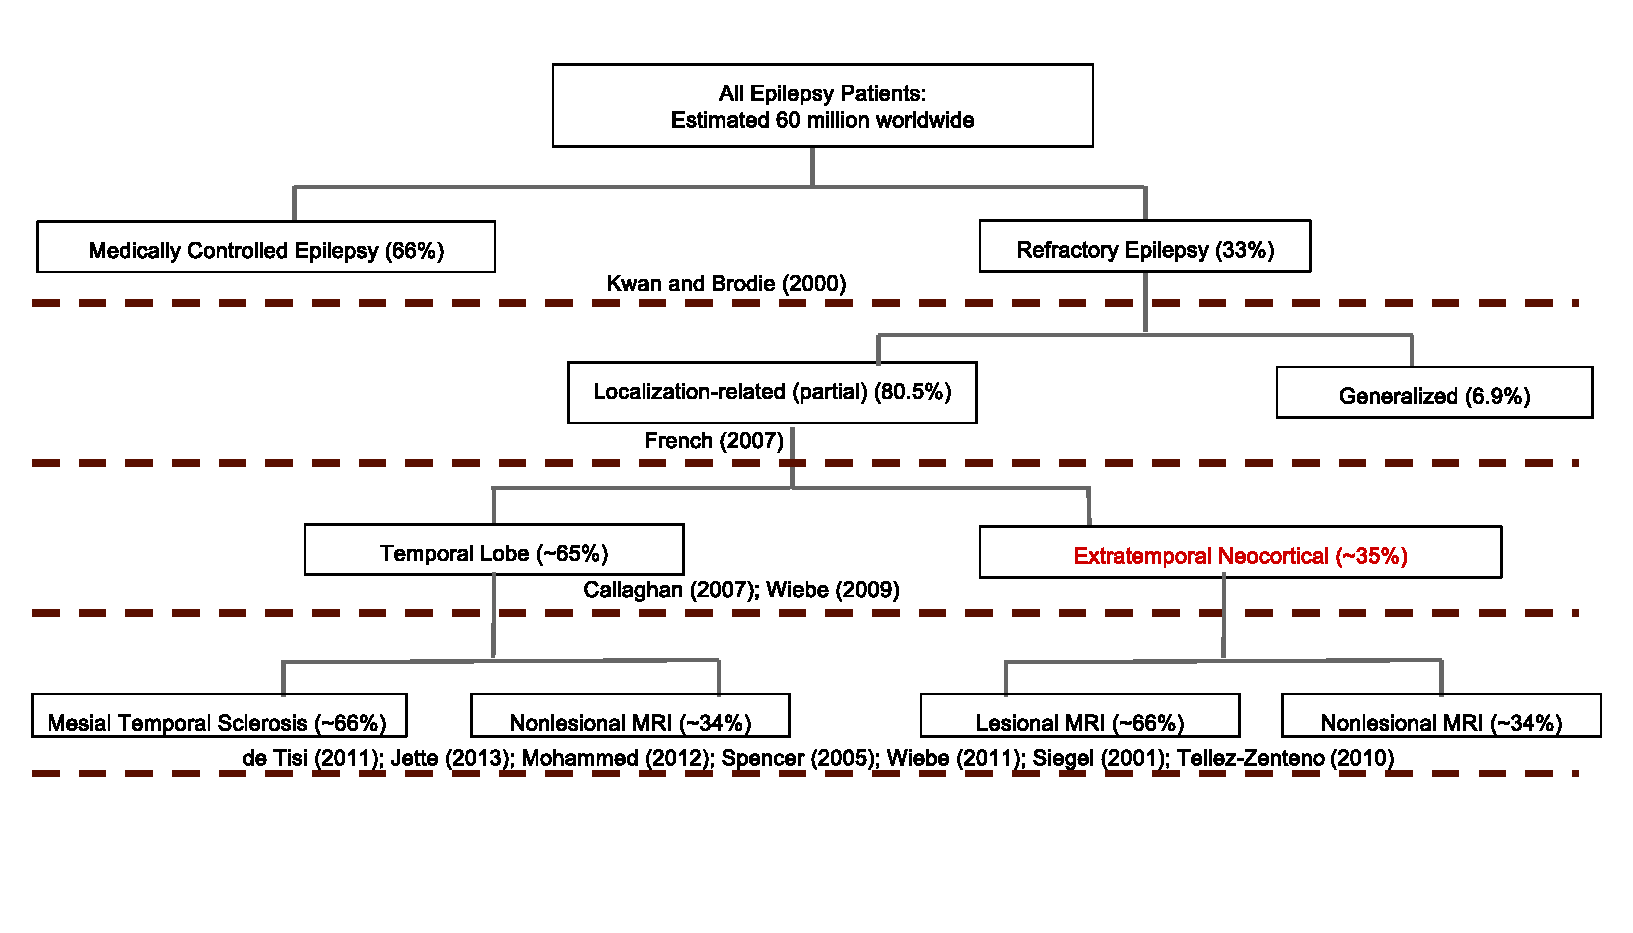
\includegraphics[width=\textwidth]{epilepsy_type}
\caption[Chart of epilepsy types]{\textbf{Population distribution of epilepsy types.} The distribution of patients with different types of epilepsies. The literature sources used to estimate population percentage is listed at each level. The focus of this work is extratemporal neocortical epilepsy, which has a prevalence of $\approx$6 million people.}
\label{epilepsy_type}
\end{figure}

\subsection{Clinical Imaging to Localize Structural and Functional Abnormalities}
While intracranial monitoring of neural activity associated with epileptic events is indispensable for identifying the seizure origin, multi-modal imaging can often identify lesions (\textbf{Fig.~\ref{typeIIfcd}}) (e.g. focal cortical dysplasia, tuberous sclerosis, other malformations of cortical development), which when resected lead to significantly better odds (2.9 times) of seizure freedom than in cases where imaging returns negative findings \cite{tellez-zenteno2010surgical}. For cases with unknown etiology, only $\approx$54\% of patients attain favorable seizure freedom (Engel score I or II) \cite{lee2005surgical}. Even in cases where no clear lesions are evident on MRI, clinicians collect a variety of imaging modalities providing orthogonal information about the epileptic network. We briefly introduce some of these imaging techniques below \cite{kuzniecky2002neuroimaging}:

\begin{figure}
\centering
\includegraphics[width=0.25\textwidth]{typeIIfcd_mri}
\caption[Example of brain lesion]{\textbf{Example of epileptogenic brain lesion.} A T2-weighted coronal FLAIR image displaying hyperintensity (white) in the inferior precuneus corresponding to a Type IIB focal cortical dysplasia, a common lesion underlying the development of focal seizures \cite{gaillard2015focal}.}
\label{typeIIfcd}
\end{figure}

\paragraph{Magnetic Resonance Imaging (MRI)}
T1 or T2-weighted imaging sequence that enables delineation of gray- and white-matter brain tissue. This imaging modality is most widely used for localizing aberrant migration of neural tissue associated with developmental disorders and investigating anatomical changes due to brain injury. Epilepsy cases with unremarkable MRI are colloquially considered \textit{non-lesional}.

\paragraph{Single Photon Emission Computed Tomography (SPECT)}
SPECT imaging is used in conjunction with an injectable radioactive tracer, which together yield a dynamic or static picture of blood perfusion through the brain. SPECT may be conducted during the ictal period to identify patterns of seizure onset and spread and, when compared to baseline interictal SPECT, can localize portions of the epileptic network in 70--90\% of patients \cite{kuzniecky2002neuroimaging}. The challenge for clinicians is accurate timing of conducting a SPECT study during seizures, which occur infrequently.

\paragraph{Positron Emission Tomography (PET)}
For epilepsy patients, PET is often used in conjunction with the radioactive tracer fluorodeoxyglucose (FDG), which together yield an estimate of metabolic activity in imaged tissue. While interictal PET has shown utility in localizing abnormalities in temporal lobe epilepsy, results are less promising for neocortical epilepsy. 

\subsection{Intracranial Monitoring of Brain Electrophysiology}
\label{subsec:ephys}
Although structural and functional imaging modalities provide significant information regarding abnormal brain tissue, the electrophysiology of neural circuits provide the clearest evidence of dysfunction when diagnosing epilepsy. A patient's neurological team will compile results from imaging and phase-I monitoring of scalp electroencephalography (EEG) and plan an invasive surgery to implant sub-dural, intracranial sensors for monitoring the electrocorticogram (ECoG) (\textbf{Fig.~\ref{intracranial_electrodes}}).  

\begin{figure}
\centering
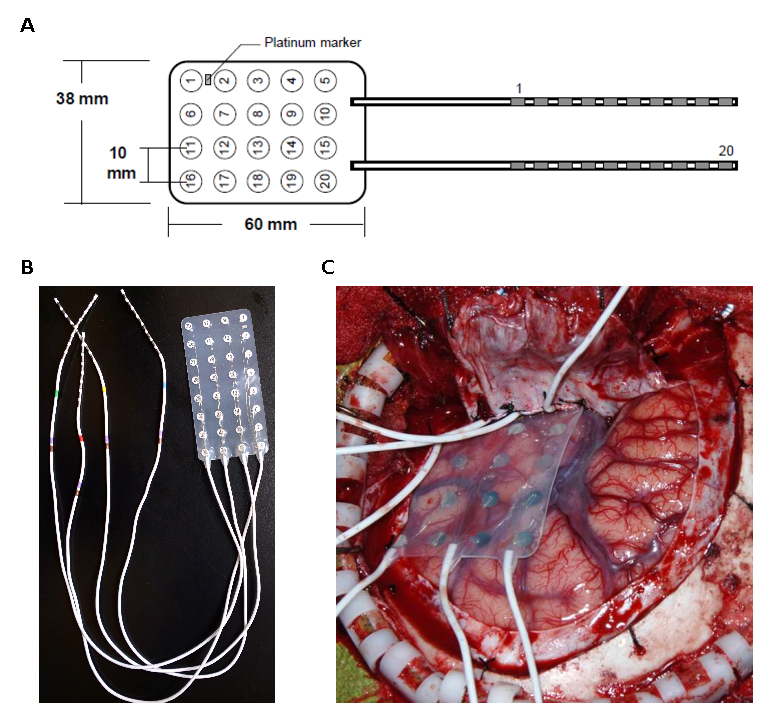
\includegraphics[width=\textwidth]{intracranial_electrodes}
\caption[Implantation of intracranial electrodes]{\textbf{Intracranial electrodes for monitoring epileptic cortex.} (\textbf{A}) Schematic of clinical-scale intracranial electrode with 20 sensors arranged in 4x5 configuration. Center-to-center distance between sensors is 10mm, and each sensor as a diameter of 4mm with 2.3mm exposed to the sub-dural cortical surface. (\textbf{B}) Photograph of a similar electrode with 32 sensors in 4x8 configuration. (\textbf{C}) Intraoperative photograph of implanted electrode in human epilepsy patient with reference to gyral, sulcal, and vascular anatomy.}
\label{intracranial_electrodes}
\end{figure}

Each sensor of an ECoG electrode is made from platinum-iridium and captures the local field potential (LFP) of neural activity from superficial layers of the neocortex \cite{buzsaki2012origin}. This LFP represents the extracellular voltage deflection from an aggregated population of neurons and is comprised of the population's synaptic activity and action potential firing patterns. Understanding the composition of the LFP is vital for connecting recorded ECoG activity to the behavior of underlying neural populations. While this is an active area of research, studies mostly agree that (i) action potentials generate a broad-band increase in the spectral power of the LFP, and (ii) spectral power in higher-frequency bands corresponds to more synchronous firing of action potentials, and (iii) higher-frequency components often phase-lock with lower-frequency components of the LFP, signifying a clear relationship between fluctuations of extracellular current and the action potentials produced by these currents \cite{buzsaki2012origin}. Below is list of frequency bands that are commonly identified in neural recordings of LFP and their physiological significance in terms of behavioral functioning:

\paragraph{Delta Band (0--4 Hz)}
Delta wave oscillations represent the slowest rhythms of LFP, and are typically recorded during the deepest stages of sleep (non-REM).

\paragraph{Theta Band (4--7 Hz)}
Theta wave oscillations are commonly observed in the hippocampus and the neocortex, although the putative functional role of this rhythm is different between the two brain regions. The hippocampal theta rhythm is typically found during behaviorally active states and have a purported relationship to learning and memory. The neocortical theta rhythm may have relevance to mechanisms of sleep and wakefulness.

\paragraph{Alpha Band (7--15 Hz)}
Alpha waves were the first discovered brain rhythm and have a strong relationship with activation of visual pathways and opening and closing of the eyes. 

\paragraph{Beta Band (15--30 Hz)}
Beta waves are believed to represent cognitive processes associated with consciousness. Additionally, beta rhythms are frequently recorded over motor cortex in conjunction with muscle contraction.

\paragraph{Low-Gamma Band (30--80 Hz)}
Rhythmic activity in low-gamma band is often connected to a wide array of cognitive tasks and is believed to play a key role in binding cognitive processes across neural systems to produce consciousness. 

\paragraph{High-Gamma Band (80--500 Hz)} 
Unlike slower neural oscillations, high-gamma band activity is purported to represent spiking activity of neural populations. High-gamma activity is of great interest to epilepsy researchers because it may be indicative of neural bursting that could initiate epileptiform events.

\subsection{Clinical Mapping of Epileptogenic Cortex}
For neurologists, rhythmic neural activity in the ECoG is not only indicative of normal brain activity, but also provides clues regarding network dysfunction. Clinicians first characterize ECoG signal properties during three major states: (i) interictal, or baseline, period of ``normal'' brain function that is at least four hours removed from a seizure, (ii) preictal period during which the brain transitions towards a seizure, and (iii) ictal period during which a critical change, away from background ECoG signal properties, occurs (i.e. the seizure).

Based on the time-varying patterns of epileptiform activity, and their spatial distributions, clinicians divide epileptic cortex into various functional regions (\textbf{Fig.~\ref{epileptic_zones}}) \cite{rosenow2001presurgical, nair2004critical}. These regions are:

\begin{figure}
\centering
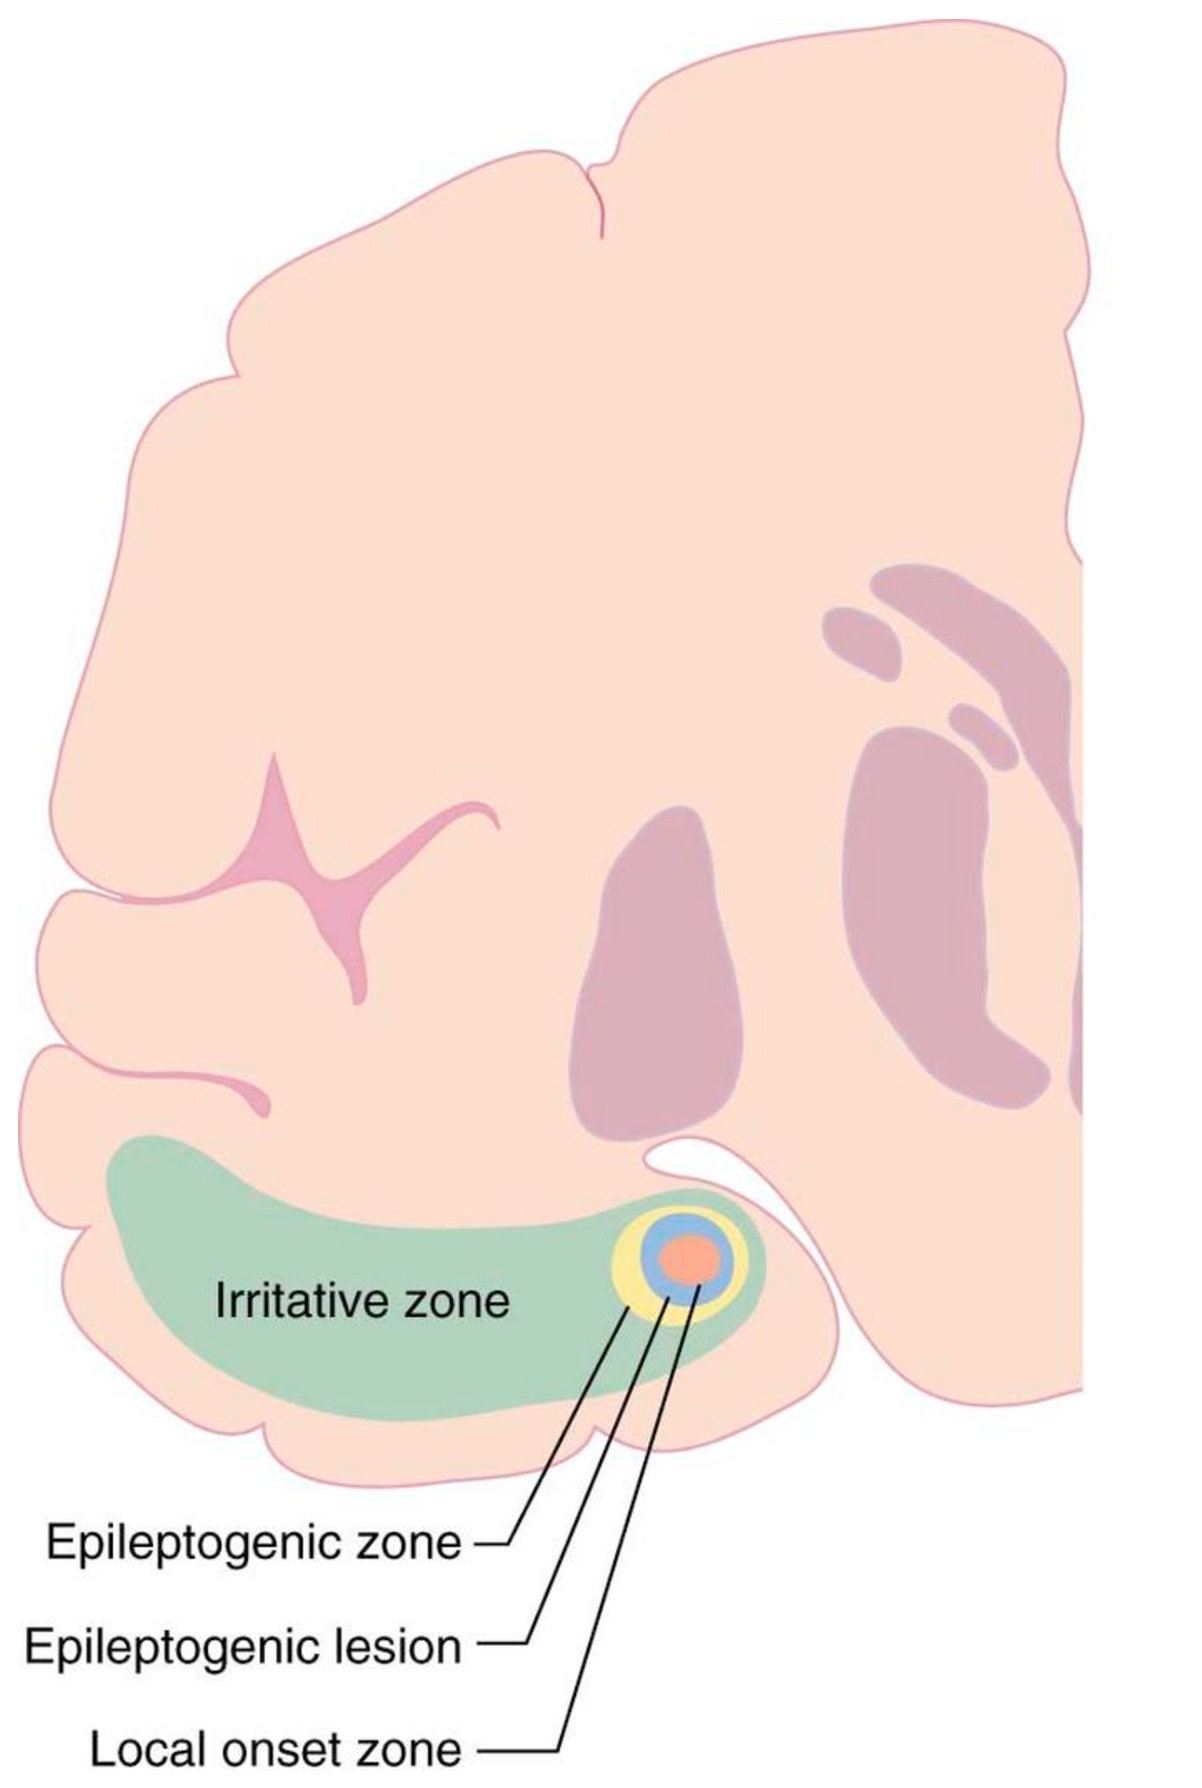
\includegraphics[width=0.5\textwidth]{epileptic_zones}
\caption[Diagram of epileptic zones]{\textbf{Organization of epileptic zones in the neocortex.} An example of the relative spatial localization of epileptic zones in the neocortex. The irritative zone displays evidence of interictal and ictal epileptiform activity that is generated in epileptogenic cortex and spreads through local pathways. The seizure-onset zone is the initial site of ictal brain activity. The epileptogenic zone is the hypothetical region that is indispensable for the generation of epileptic activity.}
\label{epileptic_zones}
\end{figure}

\paragraph{Irritative Zone}
Cortical tissue in this region generates spontaneous epileptiform activity that includes, but is not limited to, interictal spikes, spike-and-wave discharges, high-frequency oscillations, and epileptic bursts. Although these events are pathologic in nature, they do not produce clear symptoms unless a critical mass of activity is reached.

\paragraph{Seizure-Onset Zone}
This subset of the irritative zone is where clinical seizures are spontaneously generated and is the primary target for surgical resection. Ideally, the seizure-onset zone represents the initial site where the transition from preictal to ictal state occurs. However, the lack of a standardized definition between clinicians yields poor inter-rater reliability of which cortical area truly constitutes the seizure-onset zone.

\paragraph{Epileptogenic Zone}
This hypothetical region represents the full extent of cortical tissue that is capable of generating spontaneous seizures. In cases where surgical resection of the seizure-onset zone yields complete seizure freedom, the epileptogenic zone and the seizure-onset zone overlap completely. Therefore, the epileptogenic zone is a clinical construct that describes cortical regions that continue to generate seizures after surgical resection of the seizure-onset zone.

\subsection{Options for Surgical Treatment}
Until recently, surgical manipulation of the cortex was the only major option for treating drug-resistant neocortical epilepsy. Surgeons have typically resorted to resections in the frontal, parietal, and occipital lobes (5-year seizure freedom rates average $\approx$40\%), multiple subpial transections -- shallow cuts into the epileptic cortex to ``disconnect'' tissue generating seizures -- (5-year seizure freedom rates of 16\%), and callosotomy -- cutting of corpus callosum to prevent interhemispheric spread of seizures -- (5-year seizure freedom rates of 35\%) \cite{tellez-zenteno2005long-term}.  The prospect of introducing novel neurotechnologies in targeted ablative therapy and implantable devices has rejuvenated hope for a long-term solution towards controlling seizures.

Laser interstitial thermal therapy (LITT) is a minimally invasive procedure that delivers light energy, percutaneously, towards cortical tissue that requires ablation \cite{tovar-spinoza2013use, medvid2015current}. The surgical technique is image-guided and holds significant promise in epilepsy cases with identifiable focal lesions associated with seizure-onset. Furthermore, surgical cases employing LITT for epilepsy surgery have shown a reduction in cognitive deficit as compared to patients who underwent open resection \cite{drane2015better}. These studies suggest that LITT improves stereotactic control over the surgical target in epilepsy surgery.

Implantable devices that stimulate or modulate brain activity is another promising option for controlling seizures (\textbf{Fig.~\ref{implantable_devices}}) \cite{morrell2011responsive}. In contrast to early neurostimulation devices, newer devices are capable of closed-loop control that can continuously monitor ECoG for epileptic events and responsively stimulate to prevent specific events from evolving into seizures. These devices are exciting because they don't require removal of any tissue and are programmable such that therapy delivery can adjust if a patient's epilepsy characteristics change. While these devices demonstrate substantial seizure reduction, programming them requires an understanding of the electrophysiology that precipitates a patient's seizures and the optimal target for delivering stimulation. 

\begin{figure}
\centering
\includegraphics[width=\textwidth]{implantable_devices}
\caption[NeuroPace RNS Device]{\textbf{NeuroPace responsive neurostimulator device.} (\textbf{A}) The NeuroPace stimulator device and attachable electrodes for sensing and stimulating epileptic brain. (\textbf{B}) CT-scan showing an implanted NeuroPace RNS device along with the positioned sensing and stimulating electrodes.}
\label{implantable_devices}
\end{figure}

\section{What is the Epileptic Network?}
Though conventional diagnosis of epilepsy seeks to delineate brain tissue that give rise to seizures, the notion of labeling epilepsy as a network disorder is clouded and generic. Beyond structural and functional abnormalities of cortical \textit{tissue} (e.g. malformations, lesions, epileptiform spikes, high-frequency oscillations), this thesis argues that epilepsy is a dysfunction of cortical \textit{circuits} that aberrantly generate epileptic events and subsequently spread this pathologic activity to secondary brain structures. 

At the outset, we importantly distinguish between notions of structural and functional connectivity of the epileptic network. Though not the focus of this dissertation, structural connectivity describes white-matter fiber pathways between brain regions and are believed to be the primary vehicle for large-scale spreading of seizures through the brain (i.e. secondary generalization). 

\subsection{Functional Connectivity}
While structural networks describe hardwired, white-matter connections, functional networks are thought of as communication pathways between brain regions that sub-serve neurophysiologic and behavioral operation \cite{bullmore2011brain, friston2011functional, hutchison2013dynamic}. Functional pathways may be dynamic as different neural populations communicate at different points in time. Major challenges towards modeling functional networks is understanding the spatial scale of the recorded brain signal and defining cortical structures comprising \textit{nodes} and neurophysiologic phenomena that signify \textit{connections}.

For networks derived from the electrocorticogram, networks nodes are neural populations measured by intracranial sensors and network edges are statistical relationships of similarity between neural activation patterns \cite{bullmore2011brain, friston2011functional, hutchison2013dynamic}. Under this framework, signals with more similar dynamics have a stronger functional connection between them. The statistical metric used to quantify similarity between signals dictates the neurophysiologic interpretation of a connection. Briefly, we will introduce two notions of functional connectivity used in this work.

\paragraph{Broad-Band Cross-Correlation}
The cross-correlation is a measure of linear relationships between two variables accounting for a time-dependent lag between observations. That is, how much does the neural activity at node $\mb{x} $ between $t_1$ and $t_2$, linearly relate to the neural activity at node $\mb{y}$ between $t_1+\tau$ and $t_2+\tau$ for a defined lag $\tau$. For any $\tau$, cross-correlation values closer to 1, or -1, indicate strong positive, or negative, linear relationship between signals $\mb{x}$ and $\mb{y}$. Cross-correlation values approaching 0 indicate a lack of linear similarity between the two signals.  

To measure functional connectivity using the cross-correlation similarity function $\bs{\sigma}$, we compute the maximum magnitude (absolute value) value of the cross-correlation for $t$ between $t_1$ and $t_2$ over a range of $\tau$ over the span of $t_2-t_1$ (\textbf{Eqn.~\ref{eqn:xcorr}}). 
\begin{eqnarray}
    \bs{\rho}_{\mb{xy}}(t) = \underset{\tau}{\operatorname{argmax}}\:{\mathrm{E}}[(\mb{x}(t) - \mu_{\mb{x}})(\mb{y}(t+\tau) - \mu_{\mb{y}})]
    \label{eqn:xcorr}
\end{eqnarray}
This achieves a couple things: (i) accounts for transmission delays over geographical distances and volume conduction effects observed simultaneously among nearby cortical structures, and (ii) enforces a relationship between cortical structures that says, "any fluctuation in one structure that is correlated to a fluctuation in another structure implies that the two structures are functionally co-dependent." 

A prime advantage to using cross-correlation of broad-band ECoG signal, is that connectivity is not restricted to a priori determined semiology of neural activity. This point is vital in epilepsy, where clinicians are in much disagreement in the labeling of epileptiform events (i.e. what is an epileptic spike? what is a high-frequency oscillation?). Cross-correlation is robust to the shape of the neural activity, and is more concerned with identifying whether any pattern of neural activity in one cortical structure resembles a pattern of neural activity in a second cortical structure, up to a scaling in amplitude.

\paragraph{Band-Specific Coherence}
As discussed in Section \ref{subsec:ephys}, frequency-dependent structure in the ECoG signal resembles the behavior of local neural populations in the neocortex. By examining similarity of spectral power between network nodes, we can quantify functional relationships between cortical regions based on neurophysiologic behavior (i.e. whether two regions are exhibiting delta, theta, alpha, beta or gamma rhythms at the same time). 

The coherence $\Gamma$ is a normalized measure of the cross-spectral similarity $C$ between two neural signals, $\mb{x}$ and $\mb{y}$, over frequencies $f$ within a spectral band computed for time $t$ between $t_1$ and $t_2$ (\textbf{Eqns.~\ref{eqn:xspd}} and \textbf{\ref{eqn:coh}}). 
\begin{eqnarray}
    C_{\mb{xy}}(f) = {\mathrm{E}}[\int_{t_1}^{t_2}\mb{x}(t)\mathrm{e}^{-i 2 \pi ft}dt \int_{t_1}^{t_2}\mb{y}(t)\mathrm{e}^{-i 2 \pi ft}dt]
\label{eqn:xspd}
\end{eqnarray}
\begin{eqnarray}
    \bs{\Gamma}_{\mb{xy}}(f) = \frac{\abs{C_{\mb{x}\mb{y}}(f)}^2}{\abs{C_{\mb{x}\mb{x}}(f)}\abs{C_{\mb{y}\mb{y}}(f)}}
\label{eqn:coh}
\end{eqnarray}

In this thesis, we will focus on coherence of neural activity within low-gamma (30--40 Hz) and high-gamma (95--105 Hz) frequency bands. Prior work has explored the gamma band activity in ECoG, demonstrating they represent neural firing of spatially localized neural ensembles and are active during cognitive, functional tasks  \cite{crone2006high-frequency}. However, functional networks derived from coherence in gamma band is relatively unexplored, but can be a potentially powerful technique for describing hypersynchronization of more local neural populations in epileptic cortex. These studies would be an incremental push forward from prior work demonstrating micro-domains of epileptic activity \cite{worrell2008high-frequency, schevon2009spatial, stead2010microseizures, viventi2011flexible, feldt_muldoon2013spatially, weiss2013ictal}.

\subsubsection{Dynamic Network Analysis Toolbox}
To conduct many of the network analyses in this study, we developed the \textit{Dynamic Network Analysis Toolbox (DyNe)}. DyNe was developed in the Python programming language and extracts, analyzes, and presents information from sensor networks that evolve with time. DyNe emerges from the rapidly-growing field of complex networks as a toolbox for mapping multidimensional systems whose architecture changes with time. The toolbox comprises of state-of-the-art algorithms to study and visualize system dynamics in real-time (and offline), and is available at \url{https://github.com/akhambhati/dyne}.

DyNe utilizes pipelining to analyze and visualize incoming sensor data and results. A pipeline is an ordered list of modules or pipes that process incoming data in logical steps. While pipeline construction follows general rules dictating which pipes are capable of linking, the end-user has flexibility in choosing which version of a pipe to implement depending on the specific task.

For this work, we used DyNe and created two major pipelines for measuring functional networks from ECoG. The first pipeline estimates time-varying functional connectivity based on broad-band cross-correlation. The second pipeline estimates two time-varying functional networks based on spectral coherence in low-gamma and high-gamma frequency.
